\chapter{Implementation} \label{c:impl}

The VFIO implementation by Stefan Huber for Ixy.rs was used as a reference, but changed to fit the project structure and use case. The implementation for IOMMU support includes the initialization of the IOMMU, the steps needed to create mappings to the I/O Virtual Address space and the access to the device registers.

% untangle this mess
\section{Virtual Function I/O}
Virtual Function I/O (VFIO) is an IOMMU agnostic framework for exposing devices to userspace. VFIO consists of two parts, the \texttt{vfio-pci} driver and an IOMMU API. The IOMMU API can either be the type1 IOMMU API for x86 architectures or the SPAPR IOMMU API for ppc64 architectures. We will only use the type1 IOMMU API. The VFIO PCI driver can be bound to a PCI device. This allows using \texttt{mmap(2)} to map the PCI device registers into memory. The type1 VFIO IOMMU API is used for mapping and unmapping address translations in the IOMMU. Alternatively, the IOMMUFD API can be used instead of the container API, which currently is not feature complete, but will eventually replace the container-based solution \cite{vfiokerneldocs}. The layers of VFIO can be seen on \autoref{fig:layer-vfio}. VFIO practically acts like the kernel module to userspace drivers, allowing unprivileged, regulated access to physical memory and device registers.

To use vroom with the IOMMU we need to initialize the IOMMU, VFIO, DMA and the NVMe device:
\begin{enumerate}
    \item \textbf{\nameref{sec:bindvfiopci}}: Before initializing the devices, the NVMe device needs to be unbound from the kernel driver and bound to \texttt{vfio-pci}.
    \item \textbf{\nameref{sec:iommuinit}}: As the first step of the actual driver, we need to initialize the IOMMU. This is done using the VFIO IOMMU API, which is an interface for the IOMMU driver. We can get the container file descriptor with VFIO. The group needs to be assigned to the container. In this step we also can attain the device file descriptor, which can be used to read/write/\texttt{mmap} the PCIe registers through the IOMMU.
    \item \textbf{\nameref{sec:pcieconfig}}: Using the device fd, we can enable DMA by setting a bit in the PCIe command register.
    \item \textbf{\nameref{sec:nvmeinit}}: We use \texttt{mmap} to map the NVMe base address register into memory for configuring the NVMe device.
    \item \textbf{\nameref{sec:dmamapping}}: Using the container fd, we can create a mapping in the IOMMU, and therefore exposing it to the NVMe controller for DMA.
\end{enumerate}

Interaction with the VFIO interface works by using \texttt{ioctl} system calls.
\texttt{ioctl} or control device syscall, uses a file descriptor (\texttt{fd}), operation id (\texttt{op}) and optional arguments to perform actions on devices that arent covered by other system calls.
The operation ids used for VFIO are defined as constants or enums in the \texttt{vfio.h} header file in the Linux kernel. To use them in Rust, the constants need to either be defined manually or with a crate like bindgen, which automates bindings for C and C++ libraries \cite{cratebindgen}. To keep the binary and dependency list as small as possible we chose the manual implementation.
Many \texttt{ioctl} calls used for VFIO also take in a mutable reference to a struct, which is used for specific input and/or output. These structs are also defined in \texttt{vfio.h}, and can be ported over to Rust using the \texttt{\#[repr(C)]} attribute which ensures the same struct alignment as in C.

% needs more elaboration
We implement the struct \texttt{Vfio} and the enum \texttt{VfioIommu}.

\begin{lstlisting}[language=Rust,caption={Structs used to model VFIO}, label=lst:vfiostructs]
    pub struct Vfio {
        pci_addr: String,
        device_fd: RawFd,
        page_size: Pagesize,
        iommu: VfioIommu,
    }

    enum VfioIommu {
        Container {
            container_fd: RawFd,
        },
        IOMMUFD {
            ioas_id: u32,
            iommufd: RawFd,
        },
    }
\end{lstlisting}

\subsection{Groups and Containers}
VFIO works with groups and containers. Each group can contain one or multiple devices. As many devices use DMA between each other, a single IOMMU group has to be created, as these devices cannot function in an isolated environment. The other way round can also be the case, with one device exposing two interfaces, which get their own group each. Therefore, groups are the smallest unit of granularity able to function. While groups are supposed to provide the highest amount of isolation, the need for shared memory between devices often exists. This need can be solved by using containers. Containers consist of one or more groups. The groups in one container share the same I/O virtual address space created by the IOMMU, allowing both to access the same memory.
A new container can be created by opening the file \texttt{/dev/vfio/vfio}. The groups of devices bound to \texttt{vfio-pci} can be found under the path \texttt{/dev/vfio/\$GROUP}.

\subsection{Binding NVMe to \texttt{vfio-pci}}\label{sec:bindvfiopci}
To use the IOMMU for the driver, we first need to initialize the VFIO kernel module using \texttt{modprobe} and bind the \texttt{vfio-pci} driver to the NVMe device. By changing the owner of the container and group file to an unprivileged user, vroom can use the VFIO driver to create memory mappings and interact with the device without root.

\subsection{IOMMU initialization}\label{sec:iommuinit}
To initialize the IOMMU, we first need to get the container file descriptor. The container is accessible under the path \texttt{/dev/vfio/vfio}. Using the raw container file descriptor, we can use the following \texttt{ioctl} calls:

\begin{lstlisting}[language=Rust, caption={\texttt{ioctl} calls needed for IOMMU initialization}, label=lst:containerioctls]
    ioctl_unsafe!(container_fd, VFIO_GET_API_VERSION)
    ioctl_unsafe!(container_fd, VFIO_CHECK_EXTENSION, VFIO_TYPE1_IOMMU)
    ioctl_unsafe!(group_fd, VFIO_GROUP_GET_STATUS, &group_status)
    ioctl_unsafe!(group_fd, VFIO_GROUP_SET_CONTAINER, &container_fd)
    ioctl_unsafe!(container_fd, VFIO_SET_IOMMU, VFIO_TYPE1_IOMMU)
    ioctl_unsafe!(group_fd, VFIO_GROUP_GET_DEVICE_FD, pci_addr)
    ioctl_unsafe!(container_fd, VFIO_IOMMU_GET_INFO, &iommu_info)   
\end{lstlisting}

Excluding the Status and Info calls, the functionality consists of initialising the IOMMU for the device groups by setting the container on the groups, enabling Type1 for the IOMMU and fetching the device file descriptor. With the device file descriptor, we gain access to the device regions through the VFIO device API, allowing us to \texttt{mmap} the NVMe BAR into memory.
% Using \texttt{VFIO\_IOMMU\_GET\_INFO} we can see the supported pagesizes. As our IOMMU supports 4K, 2M and 1G pagesizes the field iova\_pgsizes has the value 0x40201000.

\subsection{Device register access}\label{sec:pcieconfig}
Using the \texttt{VFIO\_DEVICE\_GET\_REGION\_INFO} \texttt{ioctl} operation on the device fd, we can access the device registers. This operation requires the struct \texttt{vfio\_region\_info} as the third parameter, which needs to be initialized with a given index from \texttt{vfio.h}. After performing the syscall, the other fields, e.g. size or offset can be used to either read/write or map device registers.

We first need to enable DMA by setting a bit in the PCIe command register.
Using \texttt{VFIO\_PCI\_CONFIG\_REGION\_INDEX} as the index, we can get the offset for the PCIe configuration space address 0x0. By then adding the command register offset (0x4) we can read the 2-byte command register, or the DMA bit and write the modified bytes back into the register.

After this, we can map the NVMe BAR register to memory. This is done using the \texttt{VFIO\_PCI\_CONFIG\_REGION\_INDEX} index. Using the offset and size, we can use \texttt{mmap} to map the BAR0 register to memory.

\begin{minipage}{.95\linewidth}
    \begin{lstlisting}[language=Rust,caption={Mapping the BAR0 NVMe register to memory}, label=lst:bar0map]
let mut region_info = vfio_region_info {
    argsz: mem::size_of::<vfio_region_info>() as u32,
    flags: 0,
    index: Self::VFIO_PCI_BAR0_REGION_INDEX,
    cap_offset: 0,
    size: 0,
    offset: 0,
};

ioctl_unsafe!(
    self.device_fd,
    IoctlOperation::VFIO_DEVICE_GET_REGION_INFO,
    &mut region_info
)?;

let len = region_info.size as usize;

let ptr = mmap_unsafe!(
    ptr::null_mut(),
    len,
    libc::PROT_READ | libc::PROT_WRITE,
    libc::MAP_SHARED,
    self.device_fd,
    region_info.offset as i64
)?; 
\end{lstlisting}
\end{minipage}

\subsection{NVMe initialization}\label{sec:nvmeinit}

% more elaboration

\begin{enumerate}
    \item Allocate Admin SQ, CQ and I/O SQ, CQ
    \item Create a mapping on the IOMMU using VFIO
    \item Configure the NVMe device
    \item Pass I/O Queue addresses to NVMe device using admin queues
\end{enumerate}

\subsection{DMA (Un-)Mapping}\label{sec:dmamapping}
In order to provide a section of memory on which the device can perform DMA operations, the user needs to either allocate some memory in the processes address space or map an existing file into the process virtual address space. This can be achieved by using \texttt{mmap}. Using \texttt{mmap}'s flags we can also define the page size used. The \texttt{MAP\_HUGETLB} flag is used in conjunction with the \texttt{MAP\_HUGE\_2MB} and \texttt{MAP\_HUGE\_1GB} flags for 2MiB and 1 GiB pages respectively. By default \texttt{mmap} uses the default page size of 4KiB.
The main IOMMU work is done by then creating the map struct \texttt{vfio\_iommu\_type1\_dma\_map}. We set the DMA mapping to read and write, and provide the same IOVA as the Virtual address. By then passing it to an ioctl call with the according VFIO operation \texttt{VFIO\_IOMMU\_MAP\_DMA} we can create a mapping in the page tables of the IOMMU. This way we can give the IOVA to the NVMe controller, which it will use to access the memory through the address translation of the IOMMU.

\begin{lstlisting}[language=Rust,caption={Mapping memory for DMA}, label=lst:mapdma]
    let mut iommu_dma_map = vfio_iommu_type1_dma_map {
        argsz: mem::size_of::<vfio_iommu_type1_dma_map>() as u32,
        flags: IoctlFlag::VFIO_DMA_MAP_FLAG_READ 
                | IoctlFlag::VFIO_DMA_MAP_FLAG_WRITE,
        vaddr: ptr as u64,
        iova: ptr as u64,
        size,
    };

    ioctl_unsafe!(
        *container_fd,
        IoctlOperation::VFIO_IOMMU_MAP_DMA,
        &mut iommu_dma_map
    )?;

    let iova = iommu_dma_map.iova as usize; 
\end{lstlisting}

% improve writing
\paragraph{Unmapping DMA}
Unmapping DMA happens when the process exits, yet for performance and application reasons we implement the \texttt{unmap\_dma} function which can be used to remove a DMA mapping from the IOMMU. Using the \texttt{VFIO\_IOMMU\_UNMAP\_DMA} \texttt{ioctl} operation we can unmap the memory, and finally free it by using \texttt{munmap}.

\newpage

\subsection{I/O operations with VFIO}
After initialization, the NVMe is ready to use. A sequential, single-threaded I/O operation is shown in \autoref{fig:vroom-graph}.
\begin{figure}
    \centering
    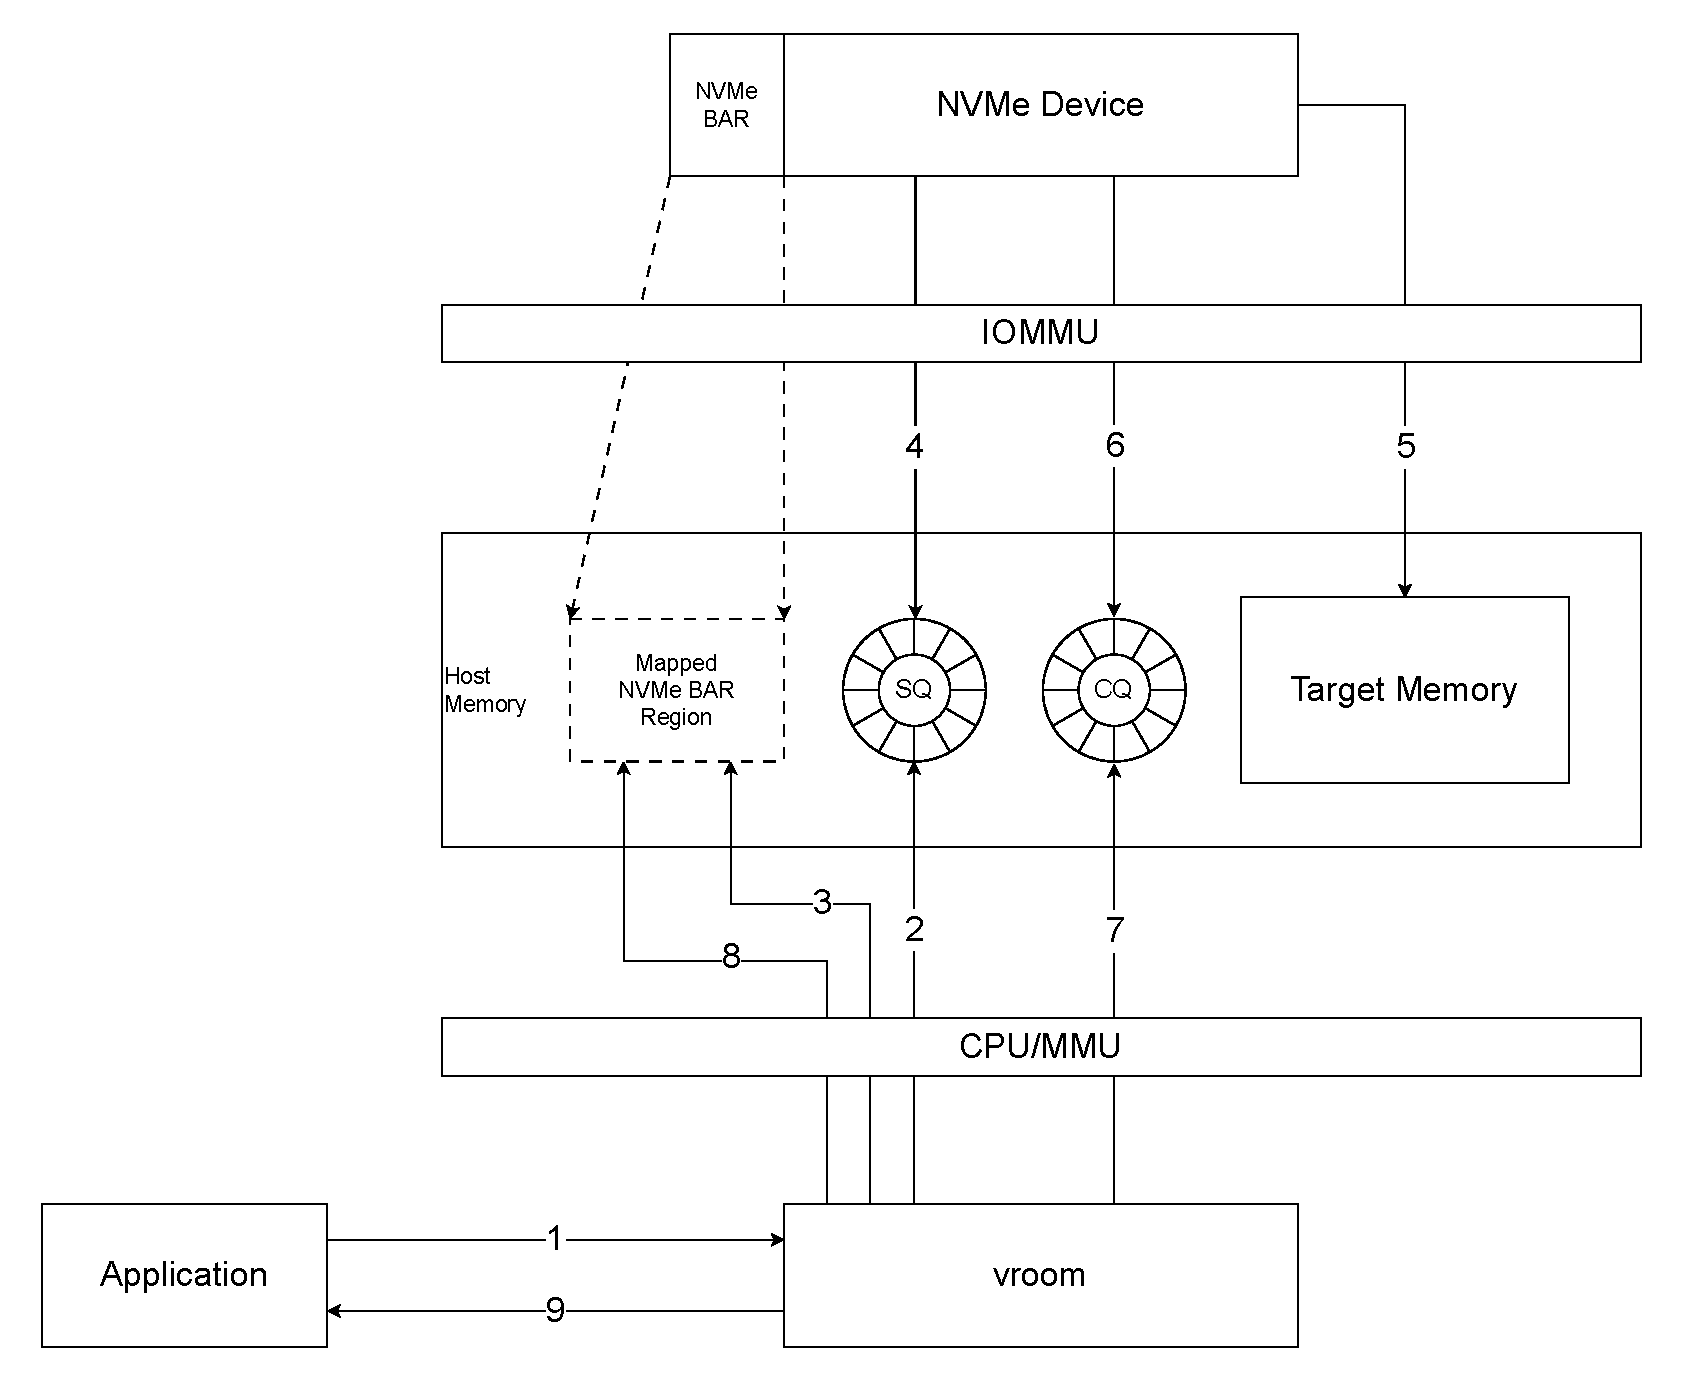
\includegraphics[width=\textwidth]{figures/vroomdiagram.pdf}
    \caption{I/O operation using vroom with enabled IOMMU}
    \label{fig:vroom-graph}
\end{figure}
The sequence of events are as followed:
\begin{enumerate}
    \item \textbf{I/O function call:} The application calls a read/write method on vroom
    \item \textbf{Command Submission:} Vroom creates a \texttt{NvmeCommand} struct and places it on the Submission Queue head.
    \item \textbf{Ring SQ Doorbell:} Vroom places the submission queue head address in the doorbell register. The doorbell register is part of the NVMe BAR region, which is mapped to memory.
    \item \textbf{Take Command:} The NVMe takes the command from the SQ.
    \item \textbf{Perform I/O:} The NVMe uses the IOMMU to access the host memory via DMA and performs the read/write command.
    \item \textbf{Complete I/O:} The NVMe places a \texttt{NvmeCompletion} struct instance on the head of the Completion Queue.
    \item \textbf{Polled CQ:} By polling the CQ, vroom can process the CQ entry.
    \item \textbf{Ring CQ Doorbell:} After processing the CQ entry, vroom rings the CQ Doorbell to notify the NVMe controller that the Completion Queue has been processed.
    \item \textbf{Notify Application:} Vroom notifies the Application of the success of the I/O operation. The application can continue running.
\end{enumerate}

\section{IOMMUFD}
The IOMMU File Descriptor user API (IOMMUFD) offers a way of controlling the IOMMU subsystem using file descriptors in user-space \cite{iommufdkerneldocs}.
IOMMUFD has only been recently added to the Linux Kernel in December 2022. E.g. Debian 12 does not include it, Fedora 40 does, but it is not enabled in the kernel configuration. Considering that it is not widely available or enabled on many distributions, our driver offers both options of using the IOMMU.
Instead of using containers or groups, IOMMUFD uses so-called I/O address spaces (IOAS) and character device file descriptors. Just like containers, IOAS can be used to provide shared memory mappings for multiple devices. The implementation of IOMMUFD is similar to VFIO, but there are some key differences.

The first change is the acquisition of the group/device and the container/iommu fd.
In VFIO, a container can be created using the file \texttt{/dev/vfio/vfio}. For IOMMUFD, first the iommu fd needs to be acquired from \texttt{/dev/iommu}. By then using the \texttt{IOMMU\_IOAS\_ALLOC} \texttt{ioctl}, a new IOAS can be allocated.
The device file descriptor, which was previously attained with \texttt{VFIO\_GROUP\_GET\_DEVICE\_FD} with the group can now be obtained through opening the character device \texttt{/dev/vfio/devices/vfioX} \cite{vfiokerneldocs}. In order to use the device with VFIO, it still has to be bound to IOMMUFD, using \texttt{VFIO\_DEVICE\_BIND\_IOMMUFD}.


The IOAS can then be assigned to the device by using \texttt{VFIO\_DEVICE\_ATTACH\_IOMMUFD\_PT}. As with containers, this operation can be performed on multiple devices for a shared IOAS. The equivalent in VFIO is \texttt{VFIO\_GROUP\_SET\_CONTAINER}.

When using VFIO with IOMMUFD, the interaction with \texttt{vfio-pci} stays the same. Primarily the whole functionality of reading, writing and mapping to the device registers is unchanged, except that the character device fd is used.

As for (un-)mapping DMA, the \texttt{IOMMU\_IOAS\_MAP} and \texttt{IOMMU\_IOAS\_UNMAP} are used.

% \begin{minipage}{\textwidth}
%     \begin{lstlisting}[language=Rust]
%         ioctl_unsafe!(cdev_fd, VFIO_DEVICE_BIND_IOMMUFD, &bind)
%         ioctl_unsafe!(iommufd, IOMMU_IOAS_ALLOC, &alloc_data)
%         ioctl_unsafe!(cdev_fd, VFIO_DEVICE_ATTACH_IOMMUFD_PT, &attach_data)
% \end{lstlisting}
% \end{minipage}

\begin{figure}[H]
    \centering
    \subcaptionbox {VFIO with Containers \label{fig:layer-vfio}} {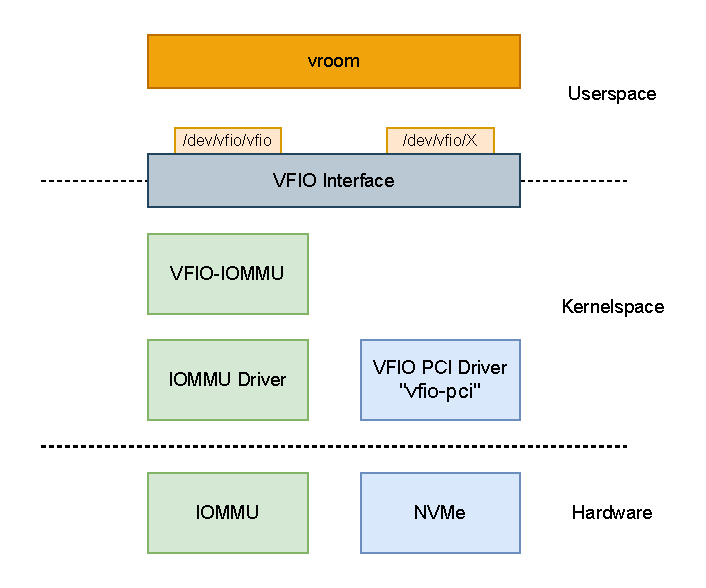
\includegraphics[width=0.67\textwidth]{figures/VFIOLayer.pdf}}
    \subcaptionbox {VFIO with IOMMUFD (IOAS) \label{fig:layer-iommufd}} {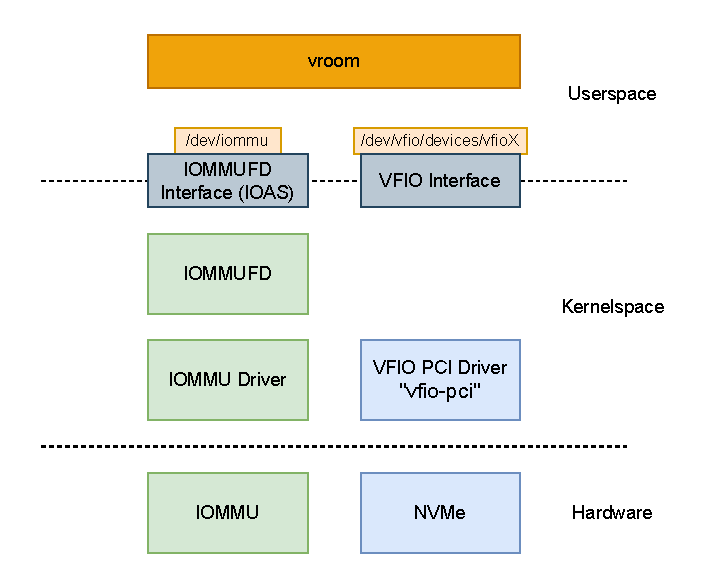
\includegraphics[width=0.67\textwidth]{figures/IOMMUFDLayer.pdf}}
    \caption{Layer diagrams of VFIO with VFIO Container API and IOMMUFD, partly adopted from \cite{dpdkiommufd}}
    \label{fig:layer}
\end{figure}

\section{Linux Systemcalls}
A variety of Linux Systemcalls (syscalls) are used in vroom. The syscalls that are used by vroom are mmap, ioctl, pread, pwrite (and mlock for the non IOMMU version). While there are crates that implement the syscall functionality, we only use the \texttt{libc} crate to avoid inflating the dependency list and executable size. As these require C-like syntax and an unsafe block in Rust, wrapper macros are used to provide locality of behaviour and secure error handling. In \autoref{lst:mmapmacro} the macro for the mmap syscall can be seen.
As part of our error handling, we introduce an error enum variant for each syscall. To not hide the inherit unsafety of these macros, we add the suffix "\_unsafe".

\begin{lstlisting}[language=Rust,caption={Syscall \texttt{mmap} macro, with own error variant}, label=lst:mmapmacro]
    #[macro_export]
    macro_rules! mmap_unsafe {
        ($addr:expr, $len:expr, $prot:expr, $flags:expr, $fd:expr, $offset:expr) => {{
            let ptr = unsafe { libc::mmap($addr, $len, $prot, $flags, $fd, $offset) };
            if ptr == libc::MAP_FAILED {
                Err(Error::Mmap {
                    error: (format!("Mmap with len {} failed", $len)),
                    io_error: (std::io::Error::last_os_error()),
                })
            } else {
                Ok(ptr)
            }
        }};
    } 
\end{lstlisting}
